\documentclass{article}
\usepackage{tikz}
\usetikzlibrary{arrows.meta}

\begin{document}

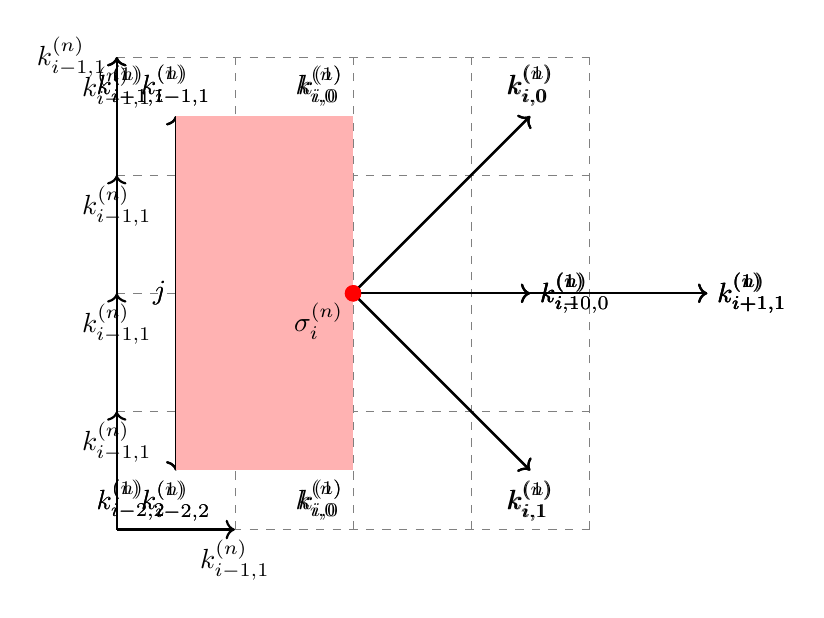
\begin{tikzpicture}[scale=1.5]
    % Draw the grid
    \draw[help lines, dashed] (-2,-2) grid (2,2);
    
    % Draw the entangling surface
    \draw[thick, ->] (-1.5,0) -- (1.5,0) node[right] {$k_{i-0,0}^{(1)}$};
    \draw[thick, ->] (-1.5,0) -- (-1.5,1.5) node[above] {$k_{i-1,1}^{(1)}$};
    \draw[thick, ->] (-1.5,0) -- (-1.5,-1.5) node[below] {$k_{i-2,2}^{(1)}$};
    \draw[thick, ->] (0,0) -- (1.5,1.5) node[above] {$k_{i,0}^{(1)}$};
    \draw[thick, ->] (0,0) -- (1.5,-1.5) node[below] {$k_{i,1}^{(1)}$};
    \draw[thick, ->] (1.5,0) -- (3,0) node[right] {$k_{i+1,1}^{(1)}$};
    
    % Draw the cut
    \fill[red!30] (-1.5,0) -- (-1.5,1.5) -- (0,1.5) -- (0,0) -- cycle;
    \fill[red!30] (-1.5,0) -- (-1.5,-1.5) -- (0,-1.5) -- (0,0) -- cycle;
    
    % Draw the intersection point
    \fill[red] (0,0) circle (2pt);
    
    % Draw the labels
    \node at (-1.5,0) [left] {$j$};
    \node at (0,0) [below left] {$\sigma_i^{(1)}$};
    \node at (0,1.5) [above left] {$k_{i,0}^{(1)}$};
    \node at (0,-1.5) [below left] {$k_{i,0}^{(1)}$};
    \node at (-1.5,1.5) [above left] {$k_{i-1,1}^{(1)}$};
    \node at (-1.5,-1.5) [below left] {$k_{i-2,2}^{(1)}$};
    \node at (1.5,0) [right] {$k_{i,1}^{(1)}$};
    \node at (3,0) [right] {$k_{i+1,1}^{(1)}$};
    
    % Draw the replica space
    \draw[thick, ->] (-2,-2) -- (-2,2) node[left] {$k_{i-1,1}^{(n)}$};
    \draw[thick, ->] (-2,-2) -- (-1,-2) node[below] {$k_{i-1,1}^{(n)}$};
    \draw[thick, ->] (-2,-2) -- (-2,-1) node[below] {$k_{i-1,1}^{(n)}$};
    \draw[thick, ->] (-2,-2) -- (-2,0) node[below] {$k_{i-1,1}^{(n)}$};
    \draw[thick, ->] (-2,-2) -- (-2,1) node[below] {$k_{i-1,1}^{(n)}$};
    \draw[thick, ->] (-2,-2) -- (-2,2) node[below] {$k_{i-1,1}^{(n)}$};
    
    % Draw the entangling surface in replica space
    \draw[thick, ->] (-1.5,0) -- (1.5,0) node[right] {$k_{i-0,0}^{(n)}$};
    \draw[thick, ->] (-1.5,0) -- (-1.5,1.5) node[above] {$k_{i-1,1}^{(n)}$};
    \draw[thick, ->] (-1.5,0) -- (-1.5,-1.5) node[below] {$k_{i-2,2}^{(n)}$};
    \draw[thick, ->] (0,0) -- (1.5,1.5) node[above] {$k_{i,0}^{(n)}$};
    \draw[thick, ->] (0,0) -- (1.5,-1.5) node[below] {$k_{i,1}^{(n)}$};
    \draw[thick, ->] (1.5,0) -- (3,0) node[right] {$k_{i+1,1}^{(n)}$};
    
    % Draw the cut in replica space
    \fill[red!30] (-1.5,0) -- (-1.5,1.5) -- (0,1.5) -- (0,0) -- cycle;
    \fill[red!30] (-1.5,0) -- (-1.5,-1.5) -- (0,-1.5) -- (0,0) -- cycle;
    
    % Draw the intersection point in replica space
    \fill[red] (0,0) circle (2pt);
    
    % Draw the labels in replica space
    \node at (-1.5,0) [left] {$j$};
    \node at (0,0) [below left] {$\sigma_i^{(n)}$};
    \node at (0,1.5) [above left] {$k_{i,0}^{(n)}$};
    \node at (0,-1.5) [below left] {$k_{i,0}^{(n)}$};
    \node at (-1.5,1.5) [above left] {$k_{i-1,1}^{(n)}$};
    \node at (-1.5,-1.5) [below left] {$k_{i-2,2}^{(n)}$};
    \node at (1.5,0) [right] {$k_{i,1}^{(n)}$};
    \node at (3,0) [right] {$k_{i+1,1}^{(n)}$};
\end{tikzpicture}

\end{document}